\input format.tex

\usepackage{graphicx}
\graphicspath{{cores/}}

\begin{document}

\vspace*{5mm}
%% 各章节
\setlength{\arrayrulewidth}{1pt}
\fontsize{9.3pt}{11pt}\selectfont
\color{gray2}

\centerline{\bf\sanhao 健康建议}

\vspace*{2mm}

\begin{LRaside}[.20]{膳食方案}
{\bf *综合您肠道菌群检测结果,为您定制以下膳食方案:}\\
{\indent 保持规律就餐的饮食习惯。控制总热量的摄入,保持正常体重。主食宜适量增加粗粮,如糙米饭、燕麦饭、全麦面等。控制动物蛋白的摄入量,宜搭配适量豆制品等植物蛋白。每天食用足量的新鲜果蔬。食用油控制在每天25克以内,以橄榄油、菜籽油等植物油为宜。食盐控制在每天6克以内。尽量减少外出就餐的次数。忌高脂、高热量饮食。忌暴饮暴食。忌烟酒。如患痛风、溃疡性结肠炎、慢性腹泻、食物不耐受等有饮食禁忌的疾病,请优先遵循疾病的饮食原则。}\\
\asidebreak %
\noindent
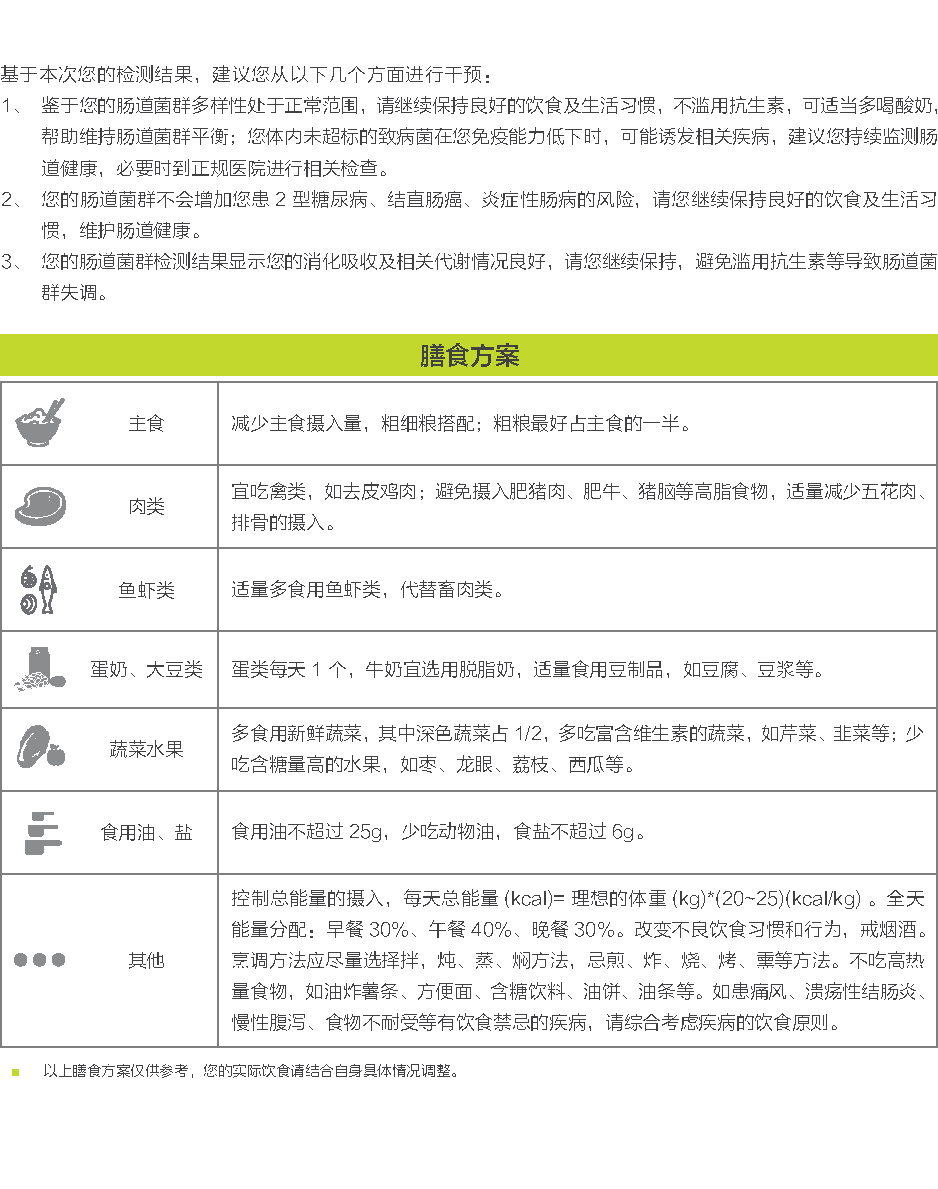
\includegraphics[width=\linewidth]{shanshifangan.pdf}

\end{LRaside}


\begin{LRaside}[.70]{肠道调节方案}
\noindent
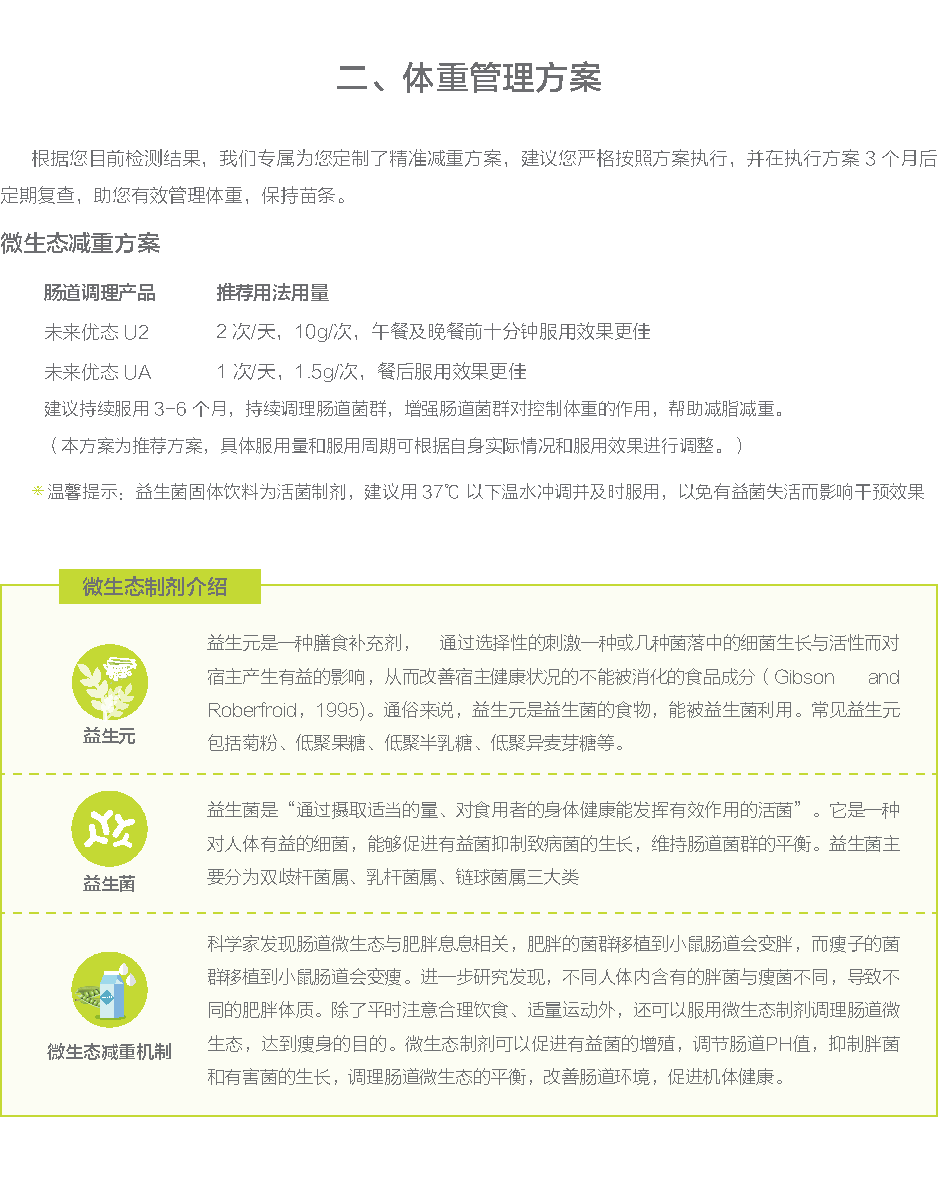
\includegraphics[width=\linewidth]{tiaojiefangan.pdf}

\asidebreak %
{\bf *综合您肠道菌群、营养功能检测结果,为您定制以下肠道调节方案:}\\
{\bf 益生元和益生菌}\\{\indent 1.可选择性补充益生元:菊粉、低聚果糖、低聚木糖等。

2.可选择性补充膳食纤维咀嚼片,能帮助您保护肠道,有益于肠道健康。

3.如患炎症性肠病、慢性腹泻,不宜服用菊粉及低聚果糖,建议选择低聚半乳糖。}\\
\end{LRaside}

\begin{LRaside}[.20]{运动方案}
{\bf *适量运动可以帮助改善肠道菌群}\\
{\indent 建议每天进行适量运动,以有氧运动为主,可根据自己的体质和喜好选择合适的运动方式,如快步走、慢跑、羽毛球、游泳、舞蹈、健身操、太极拳、爬山等,也可以选择肌肉耐力运动,如哑铃、深蹲、俯卧撑等。建议每次运动不少于30分钟,每周3-5次。尽量减少静坐时间,每间隔1小时起来活动2\textasciitilde 3分钟。}
\asidebreak %
\noindent

\includegraphics[width=\linewidth]{yundongfangan.pdf}

\end{LRaside}

%\vspace*{0.5mm}
{\noindent\qihao *以上健康建议仅供参考,您的实际饮食、保健、运动等还需结合自身具体情况。}

\end{document}
